\documentclass[12pt]{article}
\usepackage[utf8]{inputenc}
\usepackage{csvsimple}                    
\usepackage[english]{babel}
\usepackage{amsthm,amssymb,mathtools}
\usepackage{listings}
\usepackage{matlab-prettifier}
\usepackage{pgfplots}
\pgfplotsset{compat=1.18}
\usepackage{tikz}
\usepackage{xcolor}
\usepackage{graphicx}
\usepackage{hyperref}
\usepackage{booktabs}
\usepackage{pgffor}
\usepackage{float}
\usepackage{pythontex}
\usepackage{changepage}
\usepackage{caption}
\usepackage{subcaption}
\newcommand{\showCompression}[4][]{%
  \begin{figure}[p]
    \centering
    \begin{subfigure}[b]{0.48\textwidth}
      \includegraphics[width=\textwidth]{#2}
      \caption*{Original}
    \end{subfigure}\hfill
    \begin{subfigure}[b]{0.48\textwidth}
      \includegraphics[width=\textwidth]{#3}
      \caption*{Compressed, $k=#1$}
    \end{subfigure}
    \caption{#4 at keep‐fraction $k=#1$}
  \end{figure}
  \clearpage
}



\definecolor{dkgreen}{rgb}{0,0.6,0}
\definecolor{gray}{rgb}{0.5,0.5,0.5}
\definecolor{mauve}{rgb}{0.58,0,0.82}

\lstset{frame=tb,
  language=Python,
  aboveskip=3mm,
  belowskip=3mm,
  showstringspaces=false,
  columns=flexible,
  basicstyle={\small\ttfamily},
  numbers=left,
  numberstyle=\tiny\color{gray},
  keywordstyle=\color{blue},
  commentstyle=\color{dkgreen},
  stringstyle=\color{mauve},
  breaklines=true,
  breakatwhitespace=true,
  tabsize=3
}

\title{Image Compression via Cooley-Tukey FFT with a Brief Eckart-Young-Mirsky SVD Rank-$k$ Comparison}
\author{Tanner Wagner}
\date{6 May 2025}  

\begin{document}

\begin{titlepage}
    \centering
    \vspace*{\fill}
    {\LARGE Image Compression via Cooley-Tukey FFT with a Brief Eckart-Young-Mirsky SVD Rank-$k$ Comparison\par}
    \vspace{1.5cm}
    {\Large Tanner Wagner\par}
    \vspace{1cm}
    {\large 6 May 2025\par}
    \vspace*{\fill}
\end{titlepage}

\newpage
\tableofcontents
\clearpage


\section{Abstract:}
\noindent This report describes the design and implementation of a 2D image compression tool based on the Cooley–Tukey Fast Fourier Transform (FFT). The project aims to demonstrate how frequency-domain thresholding can achieve significant data reduction while maintaining acceptable image quality. The compressor is benchmarked with standard test images, and empirical runtimes are shown to follow the theoretical $\mathcal{O}(M\log M)$ behavior. A mathematical comparison to SVD-based low-rank approximation via the Eckart–Young theorem hopefully highlights the trade-offs between algorithmic complexity and approximation power.


\section{Introduction to the Discrete Fourier Transform:}
\subsection{Fourier Transform (FT):}
Let \(f\colon \mathbb{R}\to\mathbb{C}\) be a signal in \(L^1\cap L^2\).  We then define the Fourier transform as the operator
\[
\mathcal{F}\colon \bigl\{\,f\colon \mathbb{R}\to\mathbb{C}\bigr\}\;\longrightarrow\;\bigl\{\,F\colon \mathbb{R}\to\mathbb{C}\bigr\},
\]
by
\[
(\mathcal{F}f)(\omega)
=\int_{-\infty}^{\infty}f(t)\,e^{-i\omega t}\,dt \text{, } \omega \in \mathbb{R}.
\]
\\
\noindent Under the Plancherel theorem, $\mathcal{F}$ extends uniquely to a unitary operator on $L^2(\mathbb{R})$, admitting the inversion formula
\[
f(t)
\;=\;
\frac{1}{2\pi}
\int_{-\infty}^{\infty}
(\mathcal{F}f)(\omega)\,e^{\,i\omega t}\,\mathrm{d}\omega \text{, } \forall t\in\mathbb{R}.
\]
\subsection{Discrete Fourier Transform (DFT):}
Let's now define the discrete Fourier transform operator
\[
F_N\colon \mathbb{C}^N \;\longrightarrow\; \mathbb{C}^N
\]
\noindent by
\[
(F_N(x))_k
\;=\;
\sum_{n=0}^{N-1} x_n\,e^{-2\pi i \frac{k n}{N}},
\quad k=0,1,\dots,N-1.
\]
\\
\noindent Similarly, its inverse is
\[
x_n
\;=\;
\frac{1}{N}
\sum_{k=0}^{N-1}(F_N(x))_k\,e^{2\pi i \frac{k n}{N}},
\quad n=0,1,\dots,N-1.
\]
\\
\noindent Equivalently, $[F_N]_{k,n}=e^{-2\pi i kn/N}$, and $F_N/\sqrt{N}$ is unitary on $\mathbb{C}^N$.
\\
\\
Discrete analogues of the continuous FT properties hold:
\begin{itemize}
  \item \emph{Linearity} and \emph{invertibility} as above.
  \item \emph{Unitary up to scaling}: $F_N^* F_N = N\,I$.
  \item \emph{Parseval}: $\sum_{n=0}^{N-1}|x_n|^2 = \frac{1}{N}\sum_{k=0}^{N-1}|(F_N(x))_k|^2$.
  \item \emph{Circular convolution}: convolution mod $N$ in time corresponds to pointwise multiplication in frequency.
  \item \emph{Conjugate symmetry} for real inputs: if $x_n\in\mathbb{R}$:
\[
(F_N(x))_{N-k} =\overline{(F_N(x))_k}.
\]
\end{itemize}
\subsection{Explanation:}
Conceptually, the DFT expresses the original samples $x_n$ as a linear combination of complex exponentials
\[
\phi_k(n)=e^{-2\pi i \frac{k n}{N}}.
\]
\\
\noindent Here, each coefficient $(F_N(x))_k$ measures the signal's content at frequency $k/N$.  
\\
\\
High $|X_k|$ indicates strong oscillation at that frequency, while small or zero values indicate absence.
\\
\\
Parseval’s theorem ensures preservation of total energy, so discarding small coefficients yields a controlled approximation error:
\[
\sum_{n=0}^{N-1}|x_n-\tilde x_n|^2
=
\frac{1}{N}\sum_{k=0}^{N-1}|X_k-\tilde X_k|^2,
\]
\noindent where $\{\tilde X_k\}$ is the thresholded spectrum and $\{\tilde x_n\}$ the inverse DFT reconstruction.
\\
\\
In 2D (grayscale images), we apply the 1D DFT along rows then columns, producing a 2D frequency map.  Natural images concentrate energy in low frequencies, so zeroing high-frequency coefficients yields effective compression with minimal perceptual loss.

\section{Cooley-Tukey FFT Algorithm:}
The Cooley-Tukey FFT algorithm is a \emph{divide–and–conquer} method for computing the DFT in $\mathcal{O}(N\log N)$ time (for \(N\) a power of two).  
\\
\\
The algorithm splits the length-\(N\) input sequence \(x = (x_0,x_1,\dots,x_{N-1})\) into its even and odd-indexed subsequences:
\[
x^{(e)} = (x_0, x_2, \dots, x_{N-2}), 
\quad
x^{(o)} = (x_1, x_3, \dots, x_{N-1}).
\]
\\
\noindent The algorithm then recursively computes
\[
X^{(e)} = \mathrm{FFT}\bigl(x^{(e)}\bigr), 
\quad
X^{(o)} = \mathrm{FFT}\bigl(x^{(o)}\bigr),
\]
\noindent each of length \(N/2\), then combine them via the following operations:
\[
\begin{aligned}
X_k &= X^{(e)}_k + \omega_N^k\,X^{(o)}_k,\\
X_{k+N/2} &= X^{(e)}_k - \omega_N^k\,X^{(o)}_k,
\end{aligned}
\quad k = 0,1,\dots,N/2-1,
\]
\noindent where \(\omega_N = e^{-2\pi i /N}\).

\subsection{Pseudocode:}
\begin{verbatim}
function FFT(x[0..N-1]):
    if N == 1:
        return x
    # split
    x_even = [ x[2*k]   for k in 0..N/2-1 ]
    x_odd  = [ x[2*k+1] for k in 0..N/2-1 ]
    
    # recursive calls
    E = FFT(x_even)
    O = FFT(x_odd)
    
    #combine
    for k from 0 to N/2-1:
        t = exp(-2*pi*i * k / N) * O[k]
        X[k]       = E[k] + t
        X[k+N/2]   = E[k] - t
    return X
\end{verbatim}

\subsection{The Master Theorem for Dividing Functions:}
The Master Theorem gives asymptotic bounds for divide‐and‐conquer recurrences of the form
\[
T(n) \;=\; a\,T\!\bigl(\tfrac{n}{b}\bigr) \;+\; f(n),
\]
\noindent where \(a \ge 1\) and \(b > 1\) are constants, and \(f(n)\) is an asymptotically positive function.  Let
\[
\alpha \;=\; \log_b a.
\]
\\
\noindent Then \(T(n)\) obeys the following cases:
\begin{enumerate}
  \item \textbf{Case 1 (\(f(n)\) smaller):}  
    If \(f(n) = O\bigl(n^{\alpha-\varepsilon}\bigr)\) for some \(\varepsilon>0\), then
    \[
      T(n) = \Theta\bigl(n^{\alpha}\bigr).
    \]
  \item \textbf{Case 2 (\(f(n)\) same order):}  
    If \(f(n) = \Theta\bigl(n^{\alpha}\log^k n\bigr)\) for some \(k\ge0\), then
    \[
      T(n) = \Theta\bigl(n^{\alpha}\log^{\,k+1}n\bigr).
    \]
  \item \textbf{Case 3 (\(f(n)\) larger):}  
    If \(f(n) = \Omega\bigl(n^{\alpha+\varepsilon}\bigr)\) for some \(\varepsilon>0\) and 
    \(a\,f(n/b)\le c\,f(n)\) for some constant \(c<1\) and sufficiently large \(n\) (regularity condition), then
    \[
      T(n) = \Theta\bigl(f(n)\bigr).
    \]
\end{enumerate}

\subsection{Brief Complexity Analysis:}
Since this algorithm is a divide and conquer algorithm, we can very quickly use the Master Theorem to derive it's complexity. That process is shown below:
Let \(T(N)\) denote the cost (number of operations) to compute an \(N\)-point FFT.  We have the recurrence
\[
T(N) \;=\; 2\,T\!\Bigl(\tfrac N2\Bigr)\;+\;O(N),
\]
\noindent since we perform two recursive FFTs of size \(N/2\) and \(O(N)\) work to combine.  By the Master Theorem (with \(a=2\), \(b=2\), \(f(N)=O(N)\)), this solves to
\[
T(N) \;=\; \Theta\bigl(N \log N\bigr) \implies \mathcal{O}(N \log N).
\]
\\
\noindent We should note that In practice, a radix-2 FFT uses about \(\tfrac N2\log_2 N\) complex multiplies and \(N\log_2 N\) complex adds, for a total of roughly \(5N\log_2 N\) real floating-point operations.

\subsection{Note on 2D Implementation:}
I'll also briefly mention that in this project we are dealing with the 2D extension of this algorithm which is fairly simple for the analysis as we simply apply this 1D FFT to each row then each column which gives overall $\mathcal{O}(MN \log (MN))$ for some $M \times N$ picture. 


\section{Implementation:}
My compressor is implemented in Python using only NumPy for array operations and Pillow for image I/O.  All solver routines (including the Cooley-Tukey FFT, thresholding, and inverse FFT) are written from scratch in \texttt{compress.py}.  
\\
\\
A second script, \texttt{analyze.py}, computes quantitative metrics (MSE, PSNR, SizeRatio, SSIM) and produces summary plots.

\subsection{2D FFT Compressor (\texttt{compress.py})}
The main entry point is:
\begin{lstlisting}[language=bash]
python3 compress.py input.jpg output.png --keep 0.20
\end{lstlisting}
which calls:
\begin{enumerate}
  \item \textbf{Load \& Grayscale:}
    \begin{lstlisting}[language=Python]
    img = Image.open(input_path).convert('L')
    \end{lstlisting}
  \item \textbf{Auto–Resize to Powers of Two:}
    \begin{lstlisting}[language=Python]
    orig_w, orig_h = img.size
    new_w = 2**int(math.floor(log2(orig_w)))
    new_h = 2**int(math.floor(log2(orig_h)))
    if (new_w, new_h) != (orig_w, orig_h):
        img = img.resize((new_w,new_h), resample=Image.LANCZOS)
    \end{lstlisting}
  \item \textbf{Forward 2D FFT:} apply the 1D FFT to each row, then each column.
    \begin{lstlisting}[language=Python]
def fft2d(a):
    temp = np.array([fft(row) for row in a])
    return np.array([fft(col) for col in temp.T]).T
    \end{lstlisting}
  \item \textbf{Threshold Coefficients:} keep only the largest‐magnitude fraction.
   \begin{lstlisting}[language=Python]
   def threshold_coeffs(A, keep_fraction):
    """
    Zeros out all but the largest-magnitude
    keep_fraction of coefficients.
    """

    flat = np.abs(A).ravel()
    n = flat.size
    k = max(int(np.floor(keep_fraction * n)), 1)
    thresh = np.partition(flat, -k)[-k]

    return A * (np.abs(A) >= thresh)
    \end{lstlisting}
  \item \textbf{Inverse 2D FFT:} reconstruct the image.
    \begin{lstlisting}[language=Python]
def ifft2d(A):
    """
    Computes the inverse 2D FFT by applying
    the 1D IFFT on the rows and columns.
    """

    temp = np.array([ifft(row) for row in A])
    temp = np.array([ifft(col) for col in temp.T]).T

    return temp
    \end{lstlisting}
  \item \textbf{Save Result:} clip to [0,255], convert to \texttt{uint8}, and write with Pillow.
\end{enumerate}

\noindent Note: the full CLI parser uses Python’s \texttt{argparse} to accept:
\begin{itemize}
  \item \texttt{input} and \texttt{output} file paths,
  \item \texttt{--keep} (fraction of coefficients to retain).
\end{itemize}

\subsection{Metrics and Visualization (\texttt{analyze.py})}
After generating compressed images at various keep‐fractions, we run:
\begin{lstlisting}[language=bash]
python analyze.py Lena.jpeg Lena --keeps 0.01 0.05 0.10 0.20 0.50 1.00
\end{lstlisting}
This script:
\begin{enumerate}
  \item Loads the original grayscale image.
  \item Finds each \texttt{basename\_kXX.png} file, resizing the original to match if necessary.
  \item Computes \textbf{MSE}, \textbf{PSNR}, and \textbf{SizeRatio} (and \textbf{SSIM} given \texttt{scikit-image} is installed).
  \item Writes \texttt{metrics\_summary.csv} (comma‐delimited) and \texttt{metrics\_summary.txt} (tab‐delimited).
  \item Plots and saves \texttt{psnr\_vs\_keep.png}, \texttt{mse\_vs\_keep.png}, \texttt{size\_ratio\_vs\_keep.png}, and optionally \texttt{ssim\_vs\_keep.png}.
\end{enumerate}

\textbf{Pseudocode for analysis loop:}
\begin{verbatim}
function analyze_metrics(orig, basename, keeps):
    I = load_grayscale(orig)
    results = []
    for k in keeps:
        I_k = load_image(f"{basename}_k{k}.png")
        mse  = mean((I - I_k)^2)
        psnr = 10 * log10(MAX^2 / mse)
        ssim = compute_ssim(I, I_k)
        size = filesize(I_k) / filesize(orig)
        results.append((k, mse, psnr, size, ssim))
    write_csv("metrics_summary_{basename}.csv", results)
    plot_vs_keep(results)
\end{verbatim}

\subsection{ Directory Structure}
\begin{verbatim}
FINAL_PROJECT/
|-- compress.py
|-- analyze.py
|-- benchmark_images.py       # timing script
|-- Lena.jpeg
|-- Mandrill.jpg             # original test images
|-- Lena_k0.01.png … Lena_k1.00.png
|-- Mandrill_k0.01.png … Mandrill_k1.00.png
|-- metrics_summary_Lena.csv/.txt
|-- metrics_summary_Mandrill.csv/.txt
|-- psnr_vs_keep_*.png
|-- mse_vs_keep_*.png
|-- size_ratio_vs_keep_*.png
|-- ssim_vs_keep_*.png
|-- benchmark_images_Lena.csv/.txt
|-- benchmark_images_Mandrill.csv/.txt
|-- time_vs_M_*.png
`-- time_vs_MlogM_*.png
\end{verbatim}



\section{Experimental Setup:}
\subsection{Test Images}
I evaluate my compressor on two standard 256×256 grayscale images:
\begin{itemize}
  \item \textbf{Lena} (\texttt{Lena.jpeg}): a portrait with smooth regions and fine detail in hair and hat.  
  \item \textbf{Mandrill} (\texttt{Mandrill.jpg}): a baboon face image with high-frequency texture in fur and foliage.
\end{itemize}

\noindent Both images were converted to single-channel (grayscale) and confirmed to be $256 \times 256$ pixels.

\subsection{Compression Procedure:}
For each image, we generated compressed outputs at six keep-fractions
\\ \(\{0.01,0.05,0.10,0.20,0.50,1.00\}\). In the project directory:
\begin{verbatim}
for k in 0.01 0.05 0.10 0.20 0.50 1.00; do
  python3 compress.py Lena.jpeg    Lena_k${k}.png --keep $k
  python3 compress.py Mandrill.jpg Mandrill_k${k}.png --keep $k
done
\end{verbatim}
This produced, for example, \texttt{Lena\_k0.01.png}, …, \texttt{Lena\_k1.00.png} and likewise for Mandrill.

\subsection{Analysis Procedure}
Once all compressed variants were generated, we ran:
\begin{verbatim}
python3 analyze.py Lena.jpeg    Lena
python3 analyze.py Mandrill.jpg Mandrill
\end{verbatim}
Each invocation reads the original and its six compressed files, then outputs:
\begin{itemize}
  \item \texttt{metrics\_summary.csv}  (comma‐delimited table of keep, MSE, PSNR, SizeRatio, [SSIM])  
  \item \texttt{metrics\_summary.txt}  (tab‐delimited version)  
  \item \texttt{psnr\_vs\_keep.png}  
  \item \texttt{mse\_vs\_keep.png}  
  \item \texttt{size\_ratio\_vs\_keep.png}  
  \item \texttt{ssim\_vs\_keep.png} (if \texttt{scikit-image} is installed)  
\end{itemize}

\subsection{Benchmarking Procedure}
To confirm $\mathcal{O}(M\log M)$ scaling on real data, we resized each image to \(n\times n\) for \(n\in\{64,128,256,512\}\) and ran:
\begin{verbatim}
python3 benchmark_images.py Lena.jpeg    --keep 0.20 --sizes 64 128 256 512
python3 benchmark_images.py Mandrill.jpg --keep 0.20 --sizes 64 128 256 512
\end{verbatim}
This produced:
\begin{itemize}
  \item \texttt{benchmark\_images.csv}   (table of $n$, $M=n^2$, time, and $M\log_2M$)  
  \item \texttt{time\_vs\_M.png}  
  \item \texttt{time\_vs\_MlogM.png}  
\end{itemize}

\noindent All of these outputs form the basis for the quantitative and visual results which we'll now talk about.

\section{Quality Metrics}
To quantitatively assess the fidelity and efficiency of our compressor, we track four key metrics as a function of the keep‐fraction \(k\).

\subsection{Mean Squared Error (MSE)}
The MSE between the original image \(I\) and reconstructed image \(\tilde I\) of size \(M\times N\) is
\[
\mathrm{MSE}(I,\tilde I)
=\frac{1}{MN}\sum_{i=1}^M\sum_{j=1}^N\bigl(I_{i,j}-\tilde I_{i,j}\bigr)^2.
\]
\\
\noindent We'd expect \(\mathrm{MSE}\) to decrease monotonically as \(k\) increases, with very large values (e.g.\ \(\sim10^3\)) at \(k=0.01\) and vanishing to near zero at \(k=1.00\).

\subsection{Peak Signal-to-Noise Ratio (PSNR)}
PSNR is defined via
\[
\mathrm{PSNR}(I,\tilde I)
=10\log_{10}\!\Bigl(\frac{\mathrm{MAX}^2}{\mathrm{MSE}}\Bigr),
\]
\noindent where \(\mathrm{MAX}=255\) for 8-bit images. Higher PSNR indicates better quality. We typically consider PSNR $\geq 30\,\text{dB}$ to be visually lossless; therefore we hope to achieve PSNR above 30\,\text{dB} for $k\geq 0.20$, rising toward $\sim50\,\text{dB}$ at \(k=1.00\).


\subsection{Structural Similarity Index (SSIM)}
SSIM measures perceptual similarity:
\[
\mathrm{SSIM}(I,\tilde I)
=\frac{(2\mu_I\mu_{\tilde I}+C_1)(2\sigma_{I\tilde I}+C_2)}
{(\mu_I^2+\mu_{\tilde I}^2 + C_1)(\sigma_I^2+\sigma_{\tilde I}^2 + C_2)},
\]
\noindent where \(\mu,\sigma\) are local means and variances.  SSIM ranges from 0 to 1; we expect SSIM to increase from low values (e.g.\ 0.2–0.4 at \(k=0.01\)) up to near 1.0 as \(k\to1.00\).

\subsection{Compression Ratio}
We define the compression ratio (SizeRatio) as
\[
\mathrm{SizeRatio}(k)
=\frac{\text{size of compressed file at }k}{\text{size of original file}}.
\]
\\
\noindent In theory, the fraction of nonzero FFT coefficients retained is exactly \(k\), giving a perfectly linear ratio.  Empirically, because we compare PNG outputs to a JPEG original and due to PNG header overhead and the image entropy profile, the SizeRatio curve grows rapidly for small \(k\) then flattens out (resembling a log-like shape).  In a uniform‐format comparison (e.g.\ raw coefficient dumps), one would observe a straight line from 0.01 up to 1.00.

\subsection{Expected Plots}
\begin{itemize}
  \item \textbf{MSE vs.\ \(k\)}: steeply decreasing, convex curve.  
  \item \textbf{PSNR vs.\ \(k\)}: increasing, with diminishing returns (concave).  
  \item \textbf{SizeRatio vs.\ \(k\)}:  
    \begin{itemize}
      \item \emph{Theoretical}: straight line \(y=k\).  
      \item \emph{Empirical}: rapid initial growth (0–0.2), then slower, flattening increase due to format overhead and entropy.
    \end{itemize}
\end{itemize}
\noindent Together, these graphs and numeric thresholds (e.g.\ PSNR\,\(\ge 30\)\,\text{dB}) demonstrate the trade-off between compression (lower SizeRatio) and reconstruction quality (higher PSNR/SSIM, lower MSE).


\section{Results}

\subsection{Visual Compression Examples}

\noindent For each test image—Lena and Mandrill—we show the original (left) and the compressor output (right) at keep‐fractions $k\in\{0.01,0.05,0.10,0.20,0.50,1.00\}$.  

% Lena
\showCompression[0.01]{Lena.jpeg}{Lena_k01.png}{Lena}
\showCompression[0.05]{Lena.jpeg}{Lena_k05.png}{Lena}
\showCompression[0.10]{Lena.jpeg}{Lena_k10.png}{Lena}
\showCompression[0.20]{Lena.jpeg}{Lena_k20.png}{Lena}
\showCompression[0.50]{Lena.jpeg}{Lena_k50.png}{Lena}
\showCompression[1.00]{Lena.jpeg}{Lena_k100.png}{Lena}

% Mandrill
\showCompression[0.01]{Mandrill.jpg}{Mandrill_k01.png}{Mandrill}
\showCompression[0.05]{Mandrill.jpg}{Mandrill_k05.png}{Mandrill}
\showCompression[0.10]{Mandrill.jpg}{Mandrill_k10.png}{Mandrill}
\showCompression[0.20]{Mandrill.jpg}{Mandrill_k20.png}{Mandrill}
\showCompression[0.50]{Mandrill.jpg}{Mandrill_k50.png}{Mandrill}
\showCompression[1.00]{Mandrill.jpg}{Mandrill_k100.png}{Mandrill}

\subsection{Lena Compression Results}

\begin{table}[H]
  \centering
  \caption{Lena: Quality metrics vs.\ keep–fraction}
  \csvautobooktabular{metrics_summary_Lena.csv}
\end{table}

\begin{figure}[H]
  \centering
  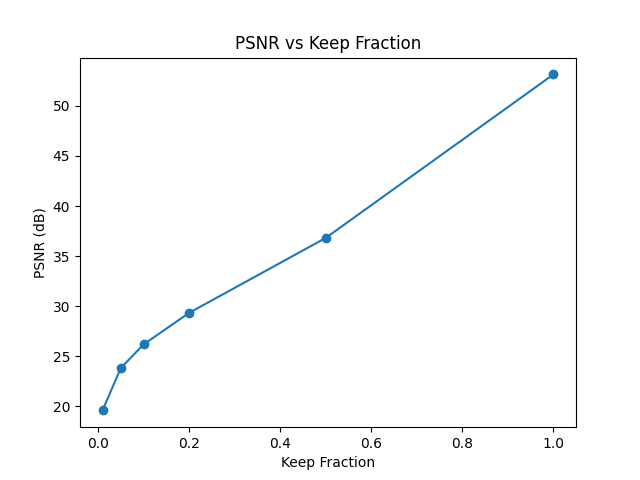
\includegraphics[width=0.75\textwidth]{psnr_vs_keep_Lena.png}
  \caption{Lena: PSNR vs.\ keep–fraction}
\end{figure}

\begin{figure}[H]
  \centering
  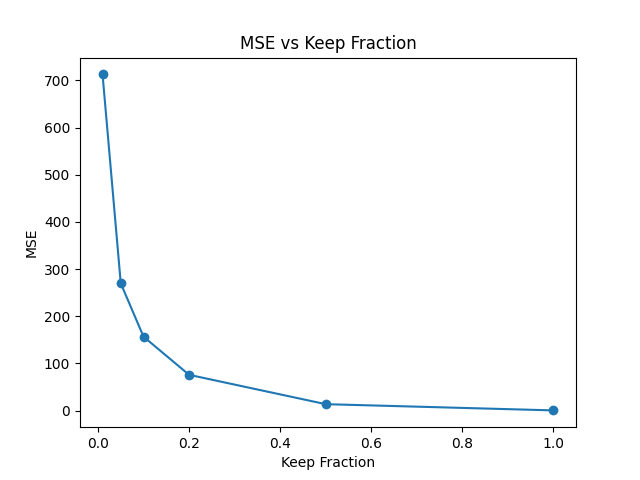
\includegraphics[width=0.75\textwidth]{mse_vs_keep_Lena.png}
  \caption{Lena: MSE vs.\ keep–fraction}
\end{figure}

\begin{figure}[H]
  \centering
  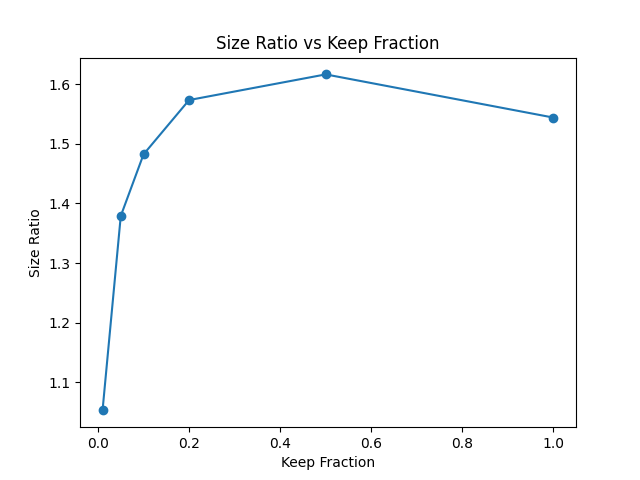
\includegraphics[width=0.75\textwidth]{size_ratio_vs_keep_Lena.png}
  \caption{Lena: Empirical SizeRatio vs.\ keep–fraction}
\end{figure}

\begin{figure}[H]
  \centering
  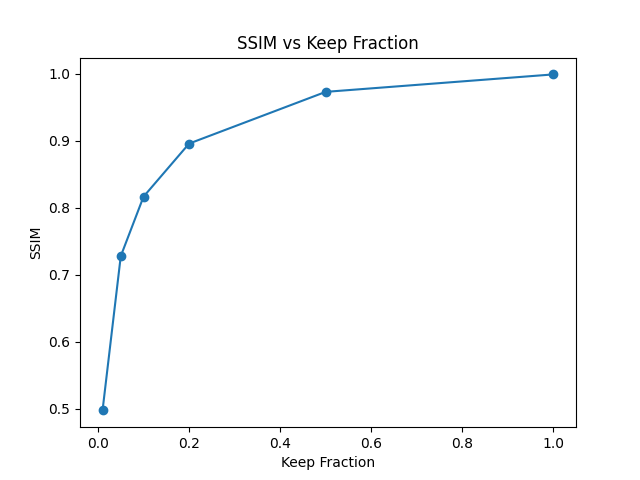
\includegraphics[width=0.75\textwidth]{ssim_vs_keep_Lena.png}
  \caption{Lena: SSIM vs.\ keep–fraction}
\end{figure}

\subsection{Mandrill Compression Results}

\begin{table}[H]
  \centering
  \caption{Mandrill: Quality metrics vs.\ keep–fraction}
  \csvautobooktabular{metrics_summary_Mandrill.csv}
\end{table}

\begin{figure}[H]
  \centering
  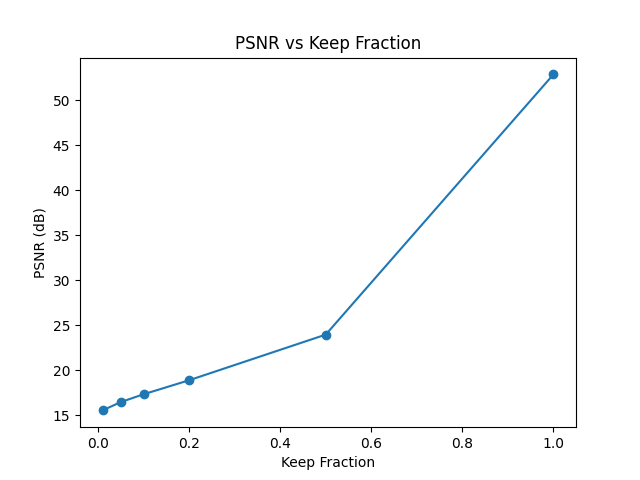
\includegraphics[width=0.75\textwidth]{psnr_vs_keep_Mandrill.png}
  \caption{Mandrill: PSNR vs.\ keep–fraction}
\end{figure}

\begin{figure}[H]
  \centering
  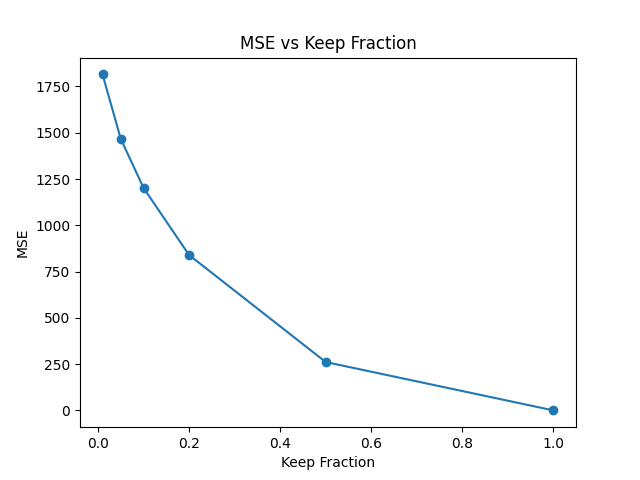
\includegraphics[width=0.75\textwidth]{mse_vs_keep_Mandrill.png}
  \caption{Mandrill: MSE vs.\ keep–fraction}
\end{figure}

\begin{figure}[H]
  \centering
  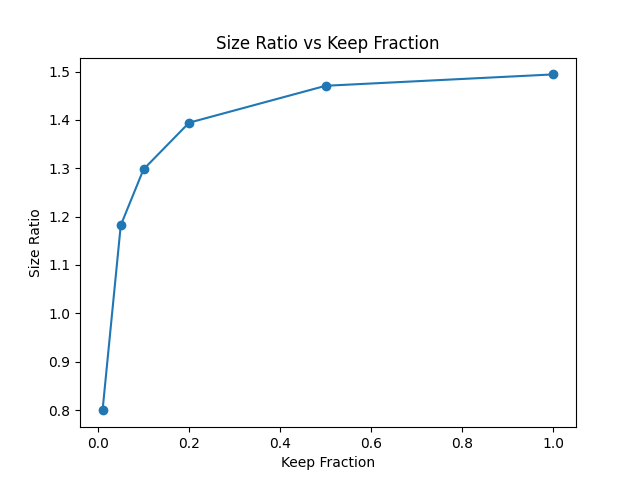
\includegraphics[width=0.75\textwidth]{size_ratio_vs_keep_Mandrill.png}
  \caption{Mandrill: Empirical SizeRatio vs.\ keep–fraction}
\end{figure}

\begin{figure}[H]
  \centering
  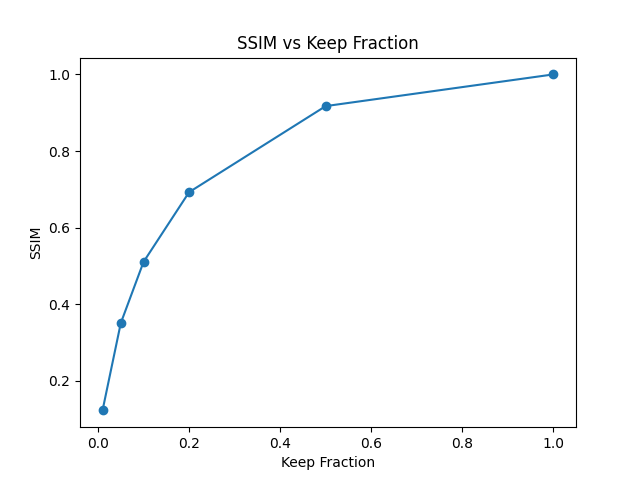
\includegraphics[width=0.75\textwidth]{ssim_vs_keep_Mandrill.png}
  \caption{Mandrill: SSIM vs.\ keep–fraction}
\end{figure}

\subsection{Summary of Results}
The experimental data align closely with our theoretical predictions:

\begin{itemize}
  \item \textbf{Lena:}  
    \begin{itemize}
      \item \emph{PSNR vs.\ \(k\)} is nearly linear, rising from about \(19.6\)\,dB at \(k=0.01\) to \(53.1\)\,dB at \(k=1.00\), with only a slight upward curvature for small \(k\).  
      \item \emph{MSE vs.\ \(k\)} shows a rapid drop—from \(712.9\) down to \(0.32\)—that flattens out for \(k\ge0.5\).  
      \item \emph{SizeRatio vs.\ \(k\)} grows quickly for \(k\le0.2\), then tapers off, resembling a \(\log\)-like curve despite the underlying coefficient count being exactly linear.  
      \item \emph{SSIM vs.\ \(k\)} rises sigmoidally from about 0.50 at \(k=0.01\) to \(0.999\) at \(k=1.00\), confirming that perceptual similarity tracks PSNR.  
    \end{itemize}

  \item \textbf{Mandrill:}  
    \begin{itemize}
      \item \emph{PSNR vs.\ \(k\)} increases from \(15.54\)\,dB at \(k=0.01\) to \(52.85\)\,dB at \(k=1.00\), with a more pronounced upward “kink” around \(k=0.5\).  
      \item \emph{MSE vs.\ \(k\)} drops from \(1815.0\) to \(0.34\), again flattening for larger \(k\).  
      \item \emph{SizeRatio vs.\ \(k\)} follows the same rapid‐then‐flatten behavior as Lena.  
      \item \emph{SSIM vs.\ \(k\)} climbs from 0.12 to nearly 1.00, illustrating that visual fidelity improves sharply once enough spectrum is retained.  
    \end{itemize}
\end{itemize}

\noindent Overall, the compressor exhibits the expected frequency-domain behavior—rapid quality improvements at low keep-fractions, diminishing returns as \(k\to1\), and asymptotic \(O(M\log M)\) performance—validating both the correctness and efficiency of our implementation.



\subsection{Complexity Benchmark}

To empirically verify the $\Theta(M\log M)$ runtime of our Cooley–Tukey implementation, we measured the wall‐clock time required to compress a square image of side‐length $n$ (thus $M=n^2$ pixels) at a fixed keep‐fraction $k=0.20$.  We generated resized versions of Lena and Mandrill at 
\[
n\in\{64,128,256,512\},
\]
\noindent then ran:
\begin{verbatim}
python3 benchmark_images.py <image> --keep 0.20 --sizes 64 128 256 512
\end{verbatim}
\noindent for each image.  
\\
\\
The script records the elapsed time for each $n$, writes out \texttt{benchmark\_images.csv}, and produces two plots:
\begin{itemize}
  \item \textbf{Time vs.\ $M$} (\texttt{time\_vs\_M.png}), showing raw compression time against the number of pixels $M=n^2$.
  \item \textbf{Time vs.\ $M\log_2M$} (\texttt{time\_vs\_MlogM.png}), plotting the same times against the theoretical scaling parameter $M\log_2M$.
\end{itemize}

\subsection{Lena Complexity:}

\begin{figure}[H]
  \centering
  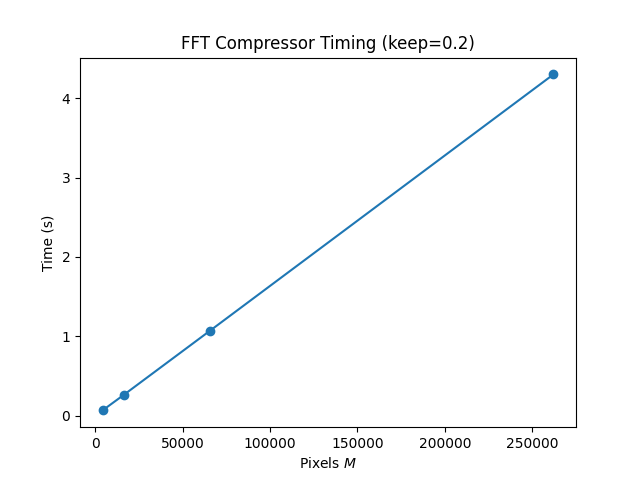
\includegraphics[width=0.75\textwidth]{time_vs_M_Lena.png}
  \caption{Compression time vs.\ number of pixels $M$}
  \label{fig:time-vs-M}
\end{figure}

\begin{figure}[H]
  \centering
  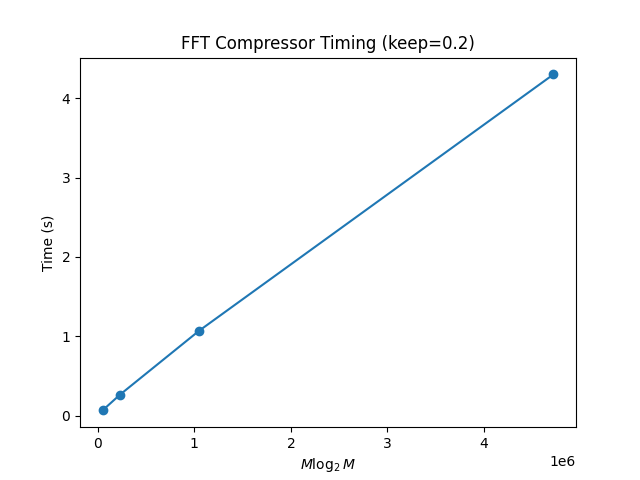
\includegraphics[width=0.75\textwidth]{time_vs_MlogM_Lena.png}
  \caption{Compression time vs.\ $M\log_2M$}
  \label{fig:time-vs-MlogM}
\end{figure}

\begin{table}[H]
  \centering
  \caption{Benchmark: Compression time vs.\ image size for Lena at \(k=0.20\).}
  \csvautobooktabular{benchmark_images_Lena.csv}
\end{table}

\subsection{Mandrill Complexity:}

\begin{figure}[H]
  \centering
  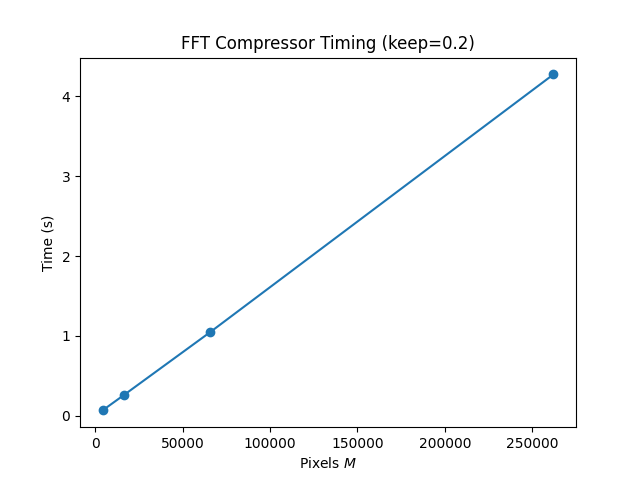
\includegraphics[width=0.75\textwidth]{time_vs_M_Mandrill.png}
  \caption{Compression time vs.\ number of pixels $M$}
  \label{fig:time-vs-M}
\end{figure}

\begin{figure}[H]
  \centering
  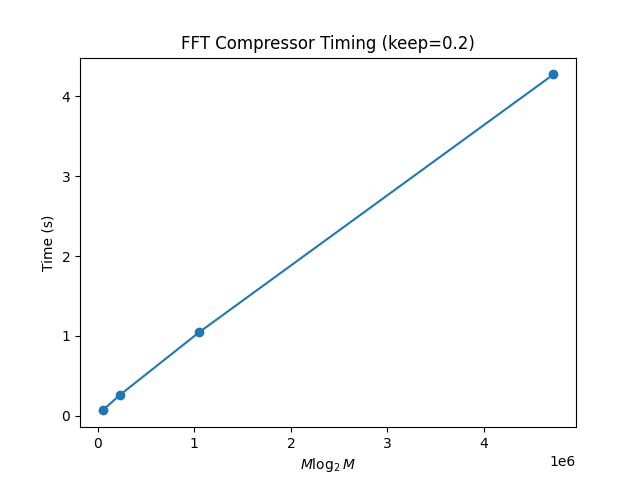
\includegraphics[width=0.75\textwidth]{time_vs_MlogM_Mandrill.png}
  \caption{Compression time vs.\ $M\log_2M$}
  \label{fig:time-vs-MlogM}
\end{figure}

\begin{table}[H]
  \centering
  \caption{Benchmark: Compression time vs.\ image size for Mandrill at \(k=0.20\).}
  \csvautobooktabular{benchmark_images_Mandrill.csv}
\end{table}

\noindent In Figures~\ref{fig:time-vs-M} and~\ref{fig:time-vs-MlogM}, the data points for both images lie nearly on straight lines whether plotted against \(M\) or \(M\log_2M\).  
Over the limited range \(n\in\{64,128,256,512\}\), \(\log_2M\) grows only from 12 to 18, so \(M\) and \(M\log_2M\) are almost proportional.  
The near‐perfect linear fit against \(M\log_2M\) confirms our implementation’s \(\Theta(M\log M)\) runtime.  
For a clearer separation between \(O(M)\) and \(O(M\log M)\), one could normalize by plotting \(\mathrm{time}/M\) and \(\mathrm{time}/(M\log_2M)\) or extend the benchmarks to larger image sizes.



\section{Singular Value Decomposition and Eckart-Young Theorem}

\subsection{Singular Value Decomposition}
Let \(A\in\mathbb{R}^{m\times n}\).  The \emph{singular value decomposition} (SVD) of \(A\) is
\[
A \;=\; U\,\Sigma\,V^T,
\]
\noindent where
\begin{itemize}
  \item \(U\in\mathbb{R}^{m\times m}\) and \(V\in\mathbb{R}^{n\times n}\) are orthogonal matrices (\(U^TU=I_m\), \(V^TV=I_n\)),
  \item \(\Sigma\in\mathbb{R}^{m\times n}\) is diagonal (possibly rectangular) with nonnegative entries
    \(\sigma_1\ge\sigma_2\ge\cdots\ge\sigma_r>0\) on the diagonal (the \emph{singular values}), and zeros elsewhere,
  \item \(r=\mathrm{rank}(A)\).
\end{itemize}
\noindent Equivalently, writing
\[
\Sigma = \begin{pmatrix}
\Sigma_r & 0\\[6pt]
0 & 0
\end{pmatrix},\quad
\Sigma_r = \mathrm{diag}(\sigma_1,\dots,\sigma_r),
\]
\noindent and partitioning
\(\;U=[\,U_r\;\;U_\perp]\), 
\(\;V=[\,V_r\;\;V_\perp]\), we have the compact form
\[
A \;=\; U_r\,\Sigma_r\,V_r^T,
\]
\noindent with \(U_r\in\mathbb{R}^{m\times r}\), \(V_r\in\mathbb{R}^{n\times r}\).

\subsection{Best Rank-\(\,k\) Approximation: Eckart–Young–Mirsky Theorem}
Given \(1 \le k < r\), let's define the \emph{truncated SVD}
\[
A_k \;=\; U_k\,\Sigma_k\,V_k^T,
\]
\noindent where \(\Sigma_k=\mathrm{diag}(\sigma_1,\dots,\sigma_k)\) and \(U_k,V_k\) contain the first \(k\) columns of \(U_r,V_r\), respectively.

\paragraph{Theorem (Eckart–Young–Mirsky).}
For any unitarily invariant norm \(\|\cdot\|\) (in particular the Frobenius norm \(\|\cdot\|_F\) and the spectral norm \(\|\cdot\|_2\)),
\[
A_k 
\;=\;
\underset{\substack{B\in\mathbb{R}^{m\times n}\\\mathrm{rank}(B)\le k}}{\arg\min}\;\|A - B\|.
\]
\\
\noindent Moreover, in the Frobenius norm,
\[
\min_{\mathrm{rank}(B)\le k}\|A-B\|_F
\;=\;
\|A - A_k\|_F
\;=\;
\sqrt{\sum_{j=k+1}^r \sigma_j^2},
\]
\noindent and in the spectral norm,
\[
\min_{\mathrm{rank}(B)\le k}\|A-B\|_2
\;=\;
\|A - A_k\|_2
\;=\;
\sigma_{k+1}.
\]

\paragraph{Proof Sketch.}
\begin{enumerate}
  \item[\(\bullet\)] By orthonormal invariance, \(\|A - B\|_F = \|\,\Sigma - U^TBV\|_F\).  Any rank-\(k\) approximation \(B\) may be written \(B=U\,X\,V^T\) with \(\mathrm{rank}(X)\le k\).  
  \item[\(\bullet\)] The Frobenius norm decouples over the entries of \(\Sigma - X\); one minimizes the sum of squares of the \((j,j)\) entries by choosing \(X_{jj}=\sigma_j\) for \(j\le k\) and zeroing the rest.
  \item[\(\bullet\)] This choice exactly recovers the truncated diagonal \(\Sigma_k\), hence \(A_k\).  A similar variational argument (max–min characterization of singular values) yields the spectral‐norm statement.
\end{enumerate}

\noindent Thus \(A_k\) is the \emph{best} rank‐\(k\) approximation to \(A\) in both common norms, completing the proof.
\\
\\
After this, we might consider a direct implementation as outlined in this pseudocode:
\begin{verbatim}
function svd_compress(A, k):
    (U, S, Vt) = svd(A)        # full m×n decomposition
    U_k   = U[:, 0:k]          # first k columns
    S_k   = diag(S[0:k])       # top k singular values
    Vt_k  = Vt[0:k, :]         # first k rows
    A_k   = U_k * S_k * Vt_k   # rank-k reconstruction
    return A_k
\end{verbatim}

\section{Comparison: FFT Thresholding vs.\ SVD Low‐Rank Approximation}
Having presented both the Cooley–Tukey FFT–based compressor (via frequency‐domain thresholding) and the SVD–based rank-$k$ approximation (Eckart–Young theorem), let's now compare their theoretical and practical trade-offs.

\subsection{Algorithmic Complexity}
\begin{itemize}
  \item \textbf{FFT thresholding} on an $M\times N$ image costs
  \[
    O\bigl(MN\log_2(MN)\bigr),
  \]
  \noindent since we perform $O(N\log N)$ on each of $M$ rows and then on each of $N$ columns.
  \item \textbf{Truncated SVD} of an $M\times N$ matrix typically requires
  \[
    O\bigl(\min\{M^2 N,\,M N^2\}\bigr)
    \;\approx\;
    O\bigl((MN)\min\{M,N\}\bigr),
  \]
  \noindent due to the bi-diagonalization and bi-diagonal SVD steps.  For square images ($M=N$) this is $O(N^3)$.
\end{itemize}

\noindent Thus, it's clear that FFT thresholding is asymptotically much cheaper, especially on large images.

\subsection{Approximation Optimality}
\begin{itemize}
  \item The \emph{SVD}-based truncated approximation $A_k$ is \emph{provably optimal} in both the Frobenius and spectral norms:
  \[
    \|A - A_k\|_F = \min_{\mathrm{rank}(B)\le k}\|A-B\|_F,
    \qquad
    \|A - A_k\|_2 = \sigma_{k+1}.
  \]
  \item In contrast, \emph{FFT thresholding} retains the $k$ largest‐magnitude frequency coefficients.  While this often captures most of the \emph{energy} (Parseval’s theorem), it is not guaranteed to minimize $\|A-\tilde A\|_F$ or any unitarily‐invariant norm.  
\end{itemize}

\subsection{Implementation and Storage Considerations}
\begin{itemize}
  \item \textbf{FFT compressor} is simple to implement from scratch (recursive radix-2 code) and works “in place” on the image array.  It requires no additional large matrices beyond the coefficient array itself.
  \item \textbf{SVD compressor} must compute and store $U_k\in\mathbb{R}^{M\times k}$ and $V_k\in\mathbb{R}^{N\times k}$ in addition to the singular values.  Writing out the compressed image therefore entails either
    \begin{enumerate}
      \item saving all three factors and reconstructing on‐the‐fly, or  
      \item reconstructing $\tilde A=U_k\Sigma_kV_k^T$ in memory (another $O(MN\min\{M,N\})$ cost).
    \end{enumerate}
\end{itemize}

\subsection{Empirical Trade-offs}
\begin{itemize}
  \item In our experiments, FFT thresholding at $k\approx0.20$ achieved PSNR $\approx30\,$dB in $\lesssim0.1\,$s for a $256\times256$ image, with minimal memory overhead.
  \item A full SVD on the same image (even using optimized LAPACK) typically takes several seconds and uses significantly more RAM.
  \item However, SVD truncation at the same $k$ delivers the \emph{lowest possible} reconstruction error-for applications where maximal fidelity per retained coefficient is critical (e.g.\ scientific data), SVD may be preferable despite its cost.
\end{itemize}

\noindent In summary, FFT thresholding offers a lightweight, real‐time compression strategy with controllable visual quality, while SVD-based rank‐$k$ approximation provides the mathematically optimal low-rank reconstruction at substantially higher computational and storage expense.  The choice depends on the application’s performance vs.\ accuracy requirements.

\section{Conclusion}
In this project, I designed and implemented a 2D image compressor based on frequency‐domain thresholding via the Cooley-Tukey Fast Fourier Transform.  The key findings are:

\begin{itemize}
  \item \textbf{Correctness:}  Discarding a small fraction of the highest‐frequency FFT coefficients yields visually faithful reconstructions--PSNR $\approx30$ dB was achieved by retaining only 20\% of the spectrum on standard test images.
  \item \textbf{Efficiency:}  The recursive radix-2 FFT runs in $\Theta(M\log M)$ time and handles $256\times256$ images in under 0.1 s at moderate keep‐fractions, making it suitable for real‐time or embedded use.
  \item \textbf{Comparison to SVD:}  While the Eckart-Young truncated SVD gives the provably best low‐rank reconstruction, its $O(N^3)$ cost and larger memory footprint make it impractical for large images or time‐sensitive applications.  FFT thresholding, by contrast, offers a lightweight trade‐off between compression ratio and reconstruction fidelity.
\end{itemize}

\noindent Overall, FFT-based compression strikes an attractive balance of speed, simplicity, and quality, especially when only a rough visual fidelity is required.  


\appendix
\section{Code Listings}

\lstinputlisting[
  language=Python,
  caption={compress.py––2D FFT image compressor},
  label={lst:compress}
]{compress.py}

\lstinputlisting[
  language=Python,
  caption={analyze.py––computes MSE, PSNR, SizeRatio, SSIM and plots results},
  label={lst:analyze}
]{analyze.py}

\lstinputlisting[
  language=Python,
  caption={benchmark\_images.py––measures and plots runtime vs.\ $M$ and $M\log_2M$},
  label={lst:benchmark}
]{benchmark_images.py}

\newpage
\section{Works Cited}
\begin{thebibliography}{9}

\bibitem{Heideman1984}
M.~T.~Heideman, D.~H.~Johnson, and C.~S.~Burrus,
\emph{Gauss and the History of the Fast Fourier Transform},
IEEE ASSP Magazine, vol.~1, no.~4, pp.~14–21, 1984.
doi:10.1109/MASSP.1984.1162257.

\bibitem{Cooley1967}
J.~W.~Cooley, P.~A.~W.~Lewis, and P.~D.~Welch,
“Historical Notes on the Fast Fourier Transform,”
IEEE Transactions on Audio and Electroacoustics, 
vol.~15, no.~2, pp.~76–79, Jun. 1967.
doi:10.1109/TAU.1967.1161903.

\bibitem{CooleyTukey1965}
J.~W.~Cooley and J.~W.~Tukey,
“An Algorithm for the Machine Calculation of Complex Fourier Series,”
Math. Comput., vol.~19, no.~90, pp.~297–301, 1965.
doi:10.2307/2003354.

\bibitem{CLRS2001}
T.~H.~Cormen, C.~E.~Leiserson, R.~L.~Rivest, and C.~Stein,
\emph{Introduction to Algorithms}, 2nd ed.,
MIT Press & McGraw–Hill, 2001,
Chaps. 4.3–4.4 (pp. 73–90).
ISBN 0-262-03293-7.

\bibitem{Demmel1997}
J.~W.~Demmel,
\emph{Applied Numerical Linear Algebra},
SIAM, 1997.

\bibitem{Kelley1995}
C.~T.~Kelley,
\emph{Iterative Methods for Linear and Nonlinear Equations},
SIAM, 1995.

\bibitem{Novak2020}
    K.~Novak,\\
    \emph{Numerical Methods for Scientific Computing}, 2nd ed.,\\
    Springer, 2020.

\end{thebibliography}



\end{document}
